\chapter{Introduction}

  \section{Overview}

    As founder and CEO of Uber, Travis Kalanick is an example of a resilient leader~\parencite{aib2015}, who stands by his principles and is comfortable with negotiation~\parencite{bhattacharya2015}. Kalanick has demonstrated on countless occasions that as an entrepreneur, he always tries to push the limits~\parencite{smith2014}, further reinforcing his risk-taking behaviour and mind-set. However, a recent scandal involving Uber's senior vice president Emil Michael raised the question of whether Kalanick's approach to leadership had fostered an insensitive, thuggish, hyper-aggressive culture within the organisation. Michael proposed that Uber start spying on journalists to dig up dirt on the personal lives of journalists who wrote negatively about the company~\parencite{withnall2014} in response to an article which highlighted the overt sexism and misogyny that Uber appeared to embrace, with direct regard to Kalanick’s gross public comments that his company should be called ``Boober'' because of the sexual attention he gets, as a result of Uber's continued growth and success~\parencite{lacy2014}. 

    \begin{figure}
      \centering
      \begin{minipage}{7cm}
        \centering
        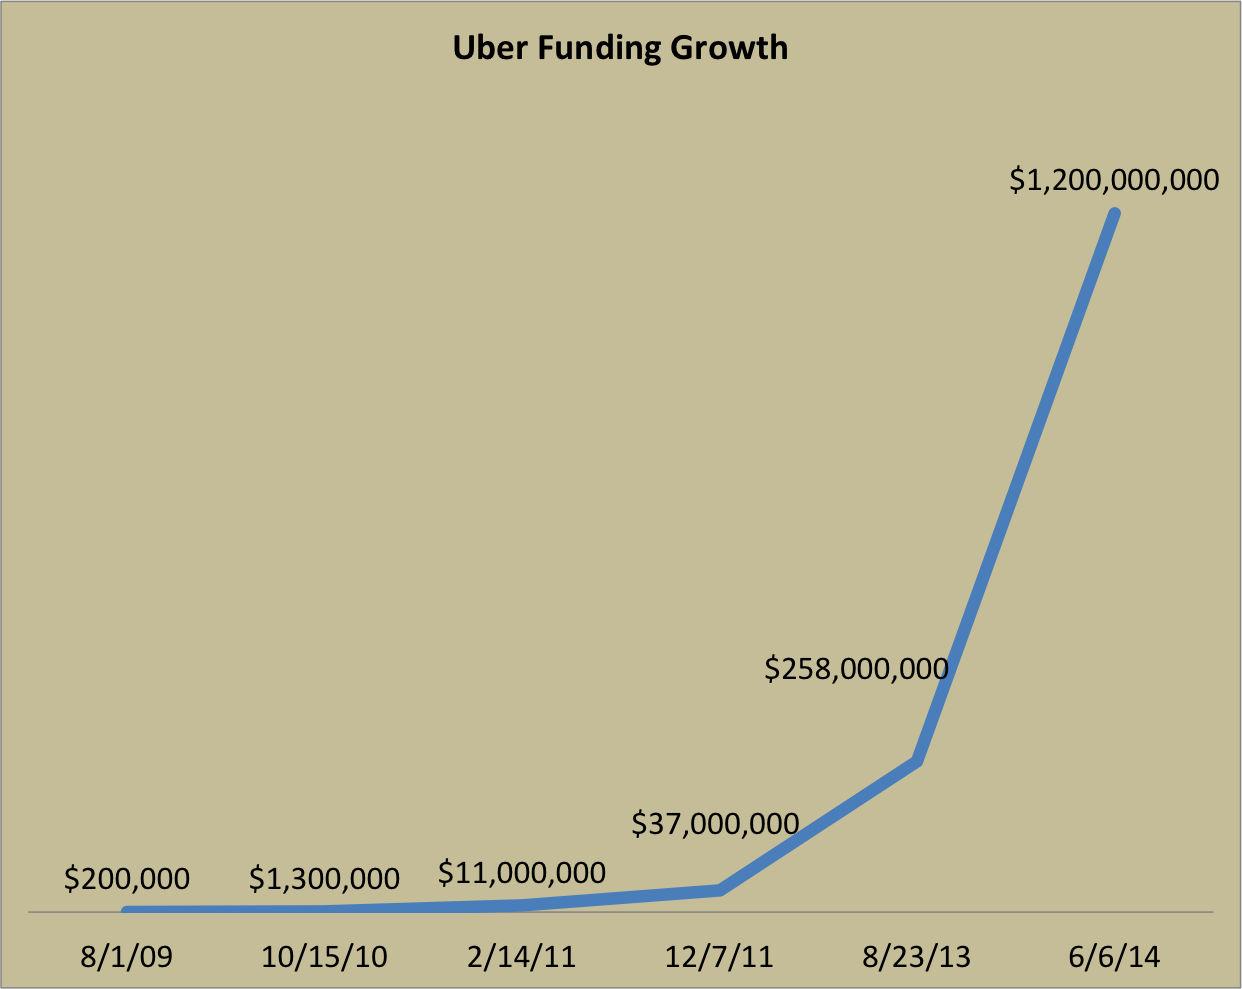
\includegraphics[width=7cm]{inc/uber_funding_growth.png}
        \caption[Uber Funding Growth]{Uber Funding Growth~\parencite{ferenstein2014}}
        \label{fig:uber_funding_growth}
      \end{minipage}
    \end{figure}

    Despite Kalanick's misgivings, Uber continues to grow exponentially see Figure~\ref{fig:uber_funding_growth}, recently completing a new round of funding that values the five-year-old company at close to \$51 billion~\parencite{macmillan2015}. An appraisal of Kalanick's leadership credentials is necessary in order to determine his contribution to the company's success. Consequently, the focus of this section is Uber's founder and CEO, Travis Kalanick -- specifically, the characteristics which assert his title as an entrepreneur. As this term ``entrepreneur'' is relevant to multiple academic contexts, such an appraisal will need to be espoused from models stemming from the fields of psychology, economics and sociology.

  \section{Psychological Conceptions}

    Psychologists tend to focus on aspects of the entrepreneur's personality, viewing them as an individual who is typically driven to experiment, perform and succeed. In addition, by starting to work on their own, entrepreneurs gain the independence required to make their own decisions~\parencite{groenewald2006}. Kalanick demonstrated such traits at an early stage when starting his first company, Scour.com, a peer-to-peer search engine which could find media content on the internet~\parencite{kessler2013}. Shortly after launching in 1998, Scour.com faced two major lawsuits over copyright infringement~\parencite{huffstutter2000}, and as the company was not able to raise money to continue operations, it filed for bankruptcy protection in order to protect itself from the impending lawsuits.

    Unperturbed by the occasion, Kalanick quickly moved on to start Red Swoosh in 2001, a relatively unsuccessful peer-to-peer file sharing company which he subsequently sold to Akamai for \$15 million in 2007. Long-term investors in Red Swoosh, asserted that Kalanick was focused, tireless and never revealed a loss of faith during this period, a testament to his hardiness~\parencite{mishkin2015}. Hardiness is a personality characteristic which is resistant to stress~\parencite{kobasa1979}. According to Cardwell \& Flanagan~\parencite{cardwell2008}, hardy individuals such as Kalanick demonstrate three characteristics:

    \begin{enumerate}
      \item Control of their lives.
      \item A strong sense of purpose combined with involvement in the world around them.
      \item A view that challenges are an opportunity to overcome and develop rather than threats or stressors.
    \end{enumerate}

    \begin{figure}
      \centering
      \begin{minipage}{7cm}
        \centering
        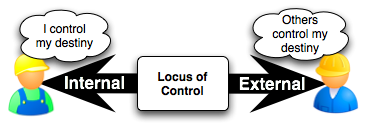
\includegraphics[width=7cm]{inc/locus_of_control.png}
        \caption[Locus of Control ]{Locus of Control~\parencite{shead2007}}
        \label{fig:locus_of_control}
      \end{minipage}
    \end{figure}

    Kalanick's positive reaction to his initial failures demonstrates that he had an internal locus of control~\parencite{rotter1966}, which was complemented by a high sense of self-efficacy~\parencite{bandura1994}. Individuals with an internal locus of control have a stronger belief that they can control their own environment, and will be more likely to exploit an entrepreneurial opportunity compared to people with an external locus of control~\parencite{engler2009}. However this requires a supplementary belief -- self-efficacy, which reflects ``confidence in the ability to exert control over one's own motivation, behaviour, and social environment''~\parencite{carey2015}. Furthermore, self-efficacy is characterised by being assured that one will accomplish a particular goal -- and to expand on this in a more present context, it can be supported by how Kalanick confidently speaks of Uber aim's to ``push rates so low that Uber rides could be a viable alternative to owning car, and possibly using public transport''~\parencite{mishkin2015}.

  \section{Economic Conceptions}
